\chapter{Implementación de la solución de lado del servidor}\label{servidor}
Los microcontroladores Arduino son usados en el diseño de sistemas embebidos para distintas funciones. El microcontrolador es un pequeño chip que posee pines con funciones de lectura y escritura, memoria, entradas y salidas. Mientras los microcontroladores han sido usados por décadas, los microcontroladores Arduino son utilizados actualmente ya que permiten ejecutar funciones electrónicas sin necesidad de conocer hardware y software integrado en estos. 
\section{Bootloader}
Dentro de las múltiples definiciones que existen con respecto al bootloader, lo más común es considerarlo como un software o firmware que reside parcialmente en la memoria no volátil del microcontrolador, como la ROM o memoria Flash. \\
En la práctica el bootloader empieza a funcionar justo después de prender el microcontrolador o después de reiniciarlo. \\
Este bootloader va a ser el que va a permitir la programación del circuito con el entorno de desarrollo Arduino (Arduino IDE) manejando de mejor manera la toma de datos por medio de las entradas análogas, el procesamiento y la comunicación.

\newpage
\section{ISP - In-System Programming}
También conocido como programación serial en circuito\cite{isp} (ICSP), es la habilidad de algunos dispositivos lógicos programables, microcontroladores y otros circuitos electrónicos de ser programados mientras están instalados en un sistema completo, no es necesario programar el chip antes de instalarlo en el sistema. Esto permite armar un circuito con todo lo que se desea y programarlo en el circuito impreso.\\
Típicamente los chips que soportan programación ISP tienen circuitería interna que genera el voltaje necesario y permite comunicarse con el programador a través de protocolo serial.
La mayoría de los dispositivos lógicos programables usan una variante del protocolo JTAG para ISP para facilitar la integración con procedimientos automatizados de pruebas.\\
JTAG (Joint Test Action Group) es una interfaz diseñada originalmente para circuitos impresos y es muy útil también como mecanismo para depuración de aplicaciones embebidas, puesto que provee una puerta trasera para acceder al sistema. El módulo de depuración permite al programador corregir errores de código y de lógica de sus sistemas.\\

\begin{figure}[H]
\centering
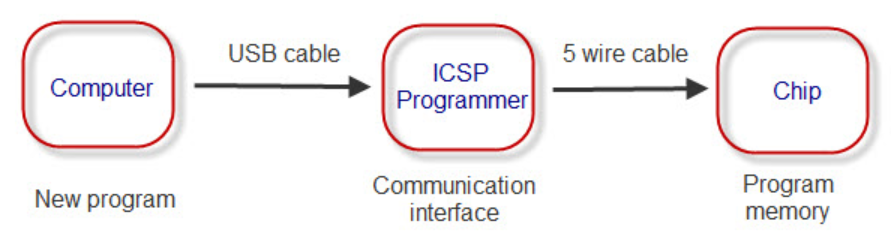
\includegraphics[scale=0.5]{figuras/firmware/isp.png}
\caption{Configuración ISP para programar un microcontrolador}
\label{isp}
\end{figure}

Se observa en la Figura \ref{isp} un simple diagrama de flujo donde es importante destacar que para poder programar un chip es necesaria una conexión de 5 cables entre un intermediario que viene a ser el programador ICSP (o ISP) y el chip (Microcontrolador).

\newpage
\section{Programación de un microcontrolador}
Para que el entorno de desarrollo Arduino reconozca el microcontrolador como una placa Arduino, es necesario grabar el bootloader en este. Se escribe el bootloader en la memoria del microcontrolador mediante la comunicación ISP que se muestra en la figura \ref{pin}.

\begin{figure}[H]
\centering
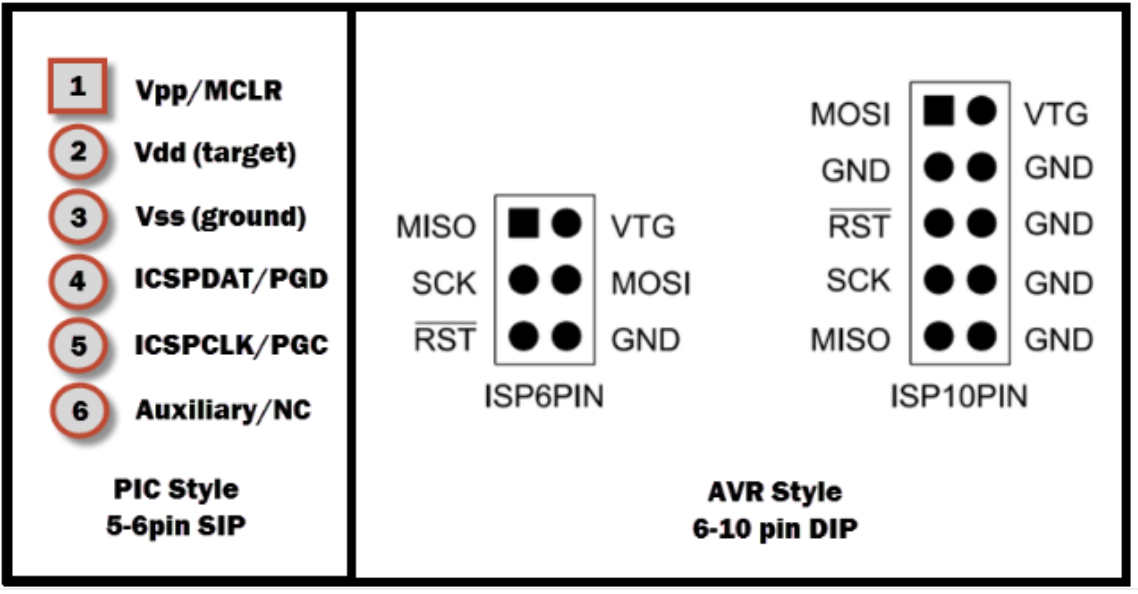
\includegraphics[scale=0.5]{figuras/firmware/pin.png}
\caption{Conector típico para programación ISP}
\label{pin}
\end{figure}

La figura \ref{pin} muestra el conector ISP que se va a encargar de cargar el bootloader en el microcontrolador.  En este caso se está utilizando la tecnología AVR (microcontrolador ATMega) la cual es usada por las placas Arduino y es por esto que se usará la configuración de 6 pines. 

\begin{figure}[H]
\centering
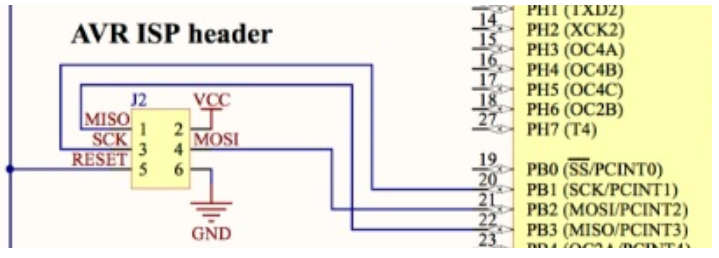
\includegraphics[scale=0.6]{figuras/firmware/eagleisp.png}
\caption{Esquemático básico MCU con ISP}
\label{eagle11}
\end{figure}

En la figura \ref{eagle11} se muestra una parte del esquemático con la configuración básica en el microcontrolador AVR.
Se puede observar el diagrama de conexión del bus con el microcontrolador. Esto se puede observar con mayor detalle en la tabla \ref{tablaisp}\\

\subsection{Programador ISP}
 Existen varias alternativas que cumplen esta función y dependen tanto del microcontrolador como del fabricante. Un microcontrolador AVR (Atmel) requiere de un programador STK500 con una interfaz serial RS232 (Existen otros programadores pero cumplen la misma función, el STK500 es el más utilizado y posee mayor compatibilidad). Para programar un microcontrolador de Microchip se requiere de un PICkit.\\ 
Una segunda alternativa es utilizar un Arduino ya programada que cumpla la función del programador. Estas vienen con un puerto ISP el cual permite cargar el bootloader en el microcontrolador. Respetando la misma conexión que se muestra en la figura \ref{eagle11}.\\

\begin{table}[H]
\centering
\begin{tabular}{| c | c | c |}
\hline
\multicolumn{1}{|c|}{\textbf{AVR ISP}}&
\multicolumn{1}{c|}{\textbf{Arduino UNO}}&
\multicolumn{1}{|c|}{\textbf{ATMega2560}}\\ \hline
1 & MISO  & Pin 22 \\ \hline
2 & VCC   & VCC    \\ \hline
3 & SCK   & PIN 20 \\ \hline
4 & MOSI  & Pin 21 \\ \hline
5 & RESET & Pin 30 \\ \hline
6 & GND   & GND    \\ \hline
\end{tabular}
\caption{Programación ISP utilizando Arduino UNO}
\label{tablaisp}
\end{table}

\section{Programación USB}
La compañía escocesa Future Technology Devices International (FTDI) está especializada en la tecnología USB (Universal Serial Bus). Esta ofrece chips encargados de transformar una conexión USB a un puerto UART y esto será fundamental a la hora de programar el diseño final con el programa en el entorno Arduino.
\newpage
\subsection{FT232RL}
El Chip FT232RL\cite{ft232} ofrece una conversión USB-UART y cuenta con 28 pines como se muestra en la figura \ref{ft232ft}.

\begin{figure}[H]
\centering
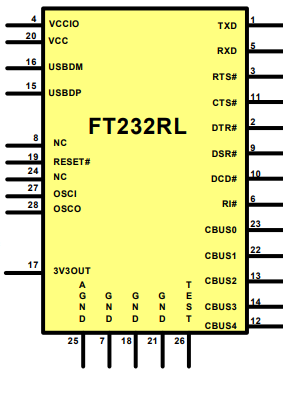
\includegraphics[scale=0.6]{figuras/firmware/ft232.png}
\caption{Chip FT232RL}
\label{ft232ft}
\end{figure}

En la tabla \ref{ft232} se muestra la descripción de los pines más importantes para la conexión del FTDI con el microcontrolador y al mismo tiempo con el USB para permitir la programación del chip. 

\begin{table}[H]
\centering
\begin{tabular}{| c | c | c | c |}
\hline
\multicolumn{1}{|c|}{\textbf{Nº Pin}}&
\multicolumn{1}{c|}{\textbf{Nombre}}&
\multicolumn{1}{|c|}{\textbf{Descripción}}\\ \hline
1  & TXD    & Transmisor de datos UART \\ \hline
5  & RXD    & Receptor de datos UART    \\ \hline
4  & VCCIO  & 1.8[V] a 5.25[V] alimentación a la interfaz UART y a los pines CBUS \\ \hline
15 & USBDP  & Conexión Data+ USB \\ \hline
16 & USBDM  & Conexión Data- USB \\ \hline
17 & 3V3OUT & Regulador de voltaje interno.    \\ \hline
22 & CBUS1  & Indicador de funcionamiento RXD   \\ \hline
23 & CBUS2  & Indicador de funcionamiento TXD    \\ \hline
\end{tabular}
\caption{Descripción de pines chip FT232RL}
\label{ft232}
\end{table}

Este chip será encargado de conectar la interfaz UART (TX y RX) con el microcontrolador además de permitir la comunicación con la conexión USB (USBDP y USBDM).\\
Al trabajar con una conexión USB se tiene conexión con VCC y GND desde el computador que está programando y este provee una alimentación de 5[V]. Este voltaje es comúnmente utilizado en los microcontroladores pero además provee un regulador de voltaje interno de 3.3[V] el cual está disponible si se está trabajando con un sistema con menor voltaje.
En caso de utilizar voltaje 3.3[V] para todo el sistema, es necesario conectar el pin 3V3OUT a VCCIO utilizando un condensador de 100[nF] como se indica en el manual. De esta forma la alimentación del microcontrolador es la misma que la alimentación FTDI para la programación UART y no se dañan las componentes.

\begin{figure}[H]
\centering
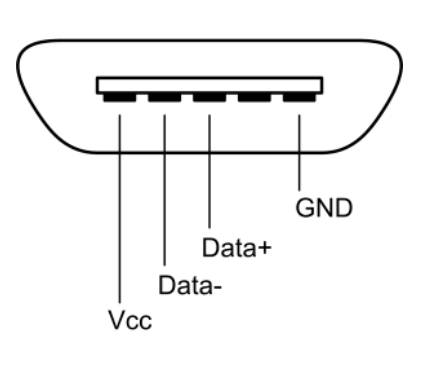
\includegraphics[scale=0.6]{figuras/firmware/usb.png}
\caption{Conector USB 2.0 Micro B}
\label{usb}
\end{figure}

Se muestra en la figura \ref{usb} las 4 conexiones que posee un conector USB, las cuales son la alimentación VCC, GND y la conexión de datos Data+ (USBDP en FT232) y Data- (USBDM en FT232). 

\newpage
\section{Programa en Arduino}

Para la programación del Arduino se trabajó en conjunto con la parte telemática del grupo. Se realizó la programación de la toma de datos de los sensores. Además de un algoritmo antirebote para pedir toma de muestras en el prototipo que luego fue sustituido por una orden emitida por la aplicación. Este código se puede observar en el anexo. En esta parte se puede observar la división de las tareas en el grupo debido a que esta memoria está enfocada al area de diseño de hardware mayoritariamente por lo que este código no se explicará en mayor profundidad.